\documentclass[10pt,adobefonts,fancyhdr,UTF8]{ctexbook}

\makeatletter
\usepackage[centering,paperwidth=180mm,paperheight=230mm,%
body={390pt,18.5cm},marginparsep=10pt,marginpar=50pt]{geometry}
\usepackage{color}
\usepackage{enumitem}
\usepackage{fancyvrb}
\usepackage{graphicx}
\usepackage[toc]{multitoc}
\usepackage{underscore}

\CTEXsetup[number={\thechapter}]{chapter}
\CTEXsetup[format+={\raggedleft}]{chapter}
\CTEXsetup[beforeskip={10pt}]{chapter}
\def\CTEX@chapter@aftername{\par} % \CTEXsetup[aftername={\par}]{chapter}
\CTEXsetup[format+={\raggedright}]{section}

\newfontfamily\urlfont{PT Sans Narrow}

\newcommand{\fn}[1]{\texttt{#1}}
\newcommand{\sfn}[1]{\texttt{\small #1}}
\newcommand{\kw}[1]{\textsf{#1}}
\newcommand{\myurl}[1]{{\urlfont #1}}
\newcommand{\mpar}[1]{\marginpar[\hfill\kaishu #1]{\kaishu #1}}
\renewcommand{\today}{\the\year-\the\month-\the\day}

\newcommand\begindot{\begin{itemize}
[itemsep=2pt plus 2pt minus 2pt,%
topsep=3pt plus 2pt minus 2pt,%
parsep=0pt plus 2pt minus 2pt]}
\newcommand\myenddot{\end{itemize}}

\newcommand\beginnum{\begin{enumerate}
[itemsep=2pt plus 2pt minus 2pt,%
topsep=3pt plus 2pt minus 2pt,%
parsep=0pt plus 2pt minus 2pt]}
\newcommand\myendnum{\end{enumerate}}

\DefineVerbatimEnvironment%
  {Code}{Verbatim}
  {fontsize=\small,baselinestretch=0.9,xleftmargin=3mm}

\raggedbottom
%\setlength{\parskip}{1ex plus .5ex minus .5ex}

\@addtoreset{footnote}{page}
%\def\@fncnsymbol#1{\ifcase#1\or ①\or ②\or ③\or
%   ④\or ⑤\or ⑥\or ⑦\or ⑧
%   \or ⑨ \else\@ctrerr\fi}
%\def\fncnsymbol#1{\expandafter\@fncnsymbol\csname c@#1\endcsname}
%\renewcommand{\thefootnote}{\fncnsymbol{footnote}}
%\renewcommand{\thefootnote}{\textbf{\color{blue}{\arabic{footnote}}}}

\makeatother

\begin{document}
\sloppy

\pagestyle{fancy}
\fancyhf{}
\fancyhead[RE]{\normalfont\small\rmfamily\nouppercase{\leftmark}}
\fancyhead[LO]{\normalfont\small\rmfamily\nouppercase{\rightmark}}
\fancyhead[LE,RO]{\thepage}
%\fancyfoot[LE,LO]{\small\normalfont\youyuan\BookTitle}

\makeatletter
\@openrightfalse
\makeatother

\frontmatter % 开始前言目录,页码用罗马数字

\thispagestyle{plain}
\begin{center}
  {\LARGE\textbf{\BookTitle}}

  \vspace{1em}
  {\large 陈硕 (giantchen@gmail.com)}

  \vspace{1ex}
  最后更新 \today

  \vspace{1em}
  \textbf{\large 版权声明}
\end{center}
\noindent 本作品采用“Creative Commons 署名-非商业性使用-相同方式共享 3.0 Unported许可协议 
(cc by-nc-sa)”进行许可。
\texttt{\small http://creativecommons.org/licenses/by-nc-sa/3.0/}

\vspace{1em}
多年之前我写过一篇书评《〈Word排版艺术〉读后感——兼谈与LaTeX的比较》
\footnote{\myurl{http://blog.csdn.net/solstice/article/details/187233}},

排版是一门大学问,我只是一名技术图书的作者,有一些初步的 \LaTeX 使用经验。
我不是专家,出版印刷的行话也不怎么会说。
本文的目的是让有志于用\LaTeX来排版自己书的人少走一些弯路。


\tableofcontents

\mainmatter % 开始正文,页码用阿拉伯数字

\graphicspath{{diagrams/}}

\chapter{环境}

\section{为什么要自己排版?}
\label{sec:whyTypesetting}

如果是纯文学著作,完全可以交给出版社去排版。
但是对于编程技术书籍,文字之间还穿插代码和图表,
那么出版社的专业排版人员很难排出符合程序员审美观的版面,
甚至有可能造成技术错误。


\begindot
\item 代码的排版,注意分页和折行。特别是Python这种缩进敏感的语言,
一般要避免在一个函数内分页,这会造成阅读困难。可以在函数定义之间分页。

\item 写作与排版一体化,作者可以适当改写内容,让版面更美观。
例如,假如一个函数最后一行那个花括号被挤到了下一页第一行,这就很难看。
这时可以考虑临时改变代码的缩进(从BSD风格改为K\&R风格),从而节省一两行空间,
让花括号落在本页。另外也可以稍微改变说法,避免段尾孤字成行。

\item 文责自负,防止误改。例如我为某本书写的序言,其中提到旧的 boost \fn{RegEx}
\kw{class} 和新的 \fn{regex} \kw{class} 在线程安全性方面的不同。
这本书第二版再用这篇序言的时候被编辑“统一大小写”改为 \fn{RegEx},
整段话也就失去意义了。
\myenddot


\section{为什么要用\LaTeX排版?}
\begindot
\item \LaTeX 不会自作聪明地自动更正,例如句首字母大写
(关键字 \kw{double} 变为 \kw{Double}),
单词头两个字母大写(\fn{IUnknown} 变为 \fn{Iunknown}),
括号匹配(“[begin, end)”变为“[begin, end]”)等等。
Word 可以关闭自动更正,但是一旦整个流程(作者、编辑、校对、出片)中有一个人的设置不同,
稿子就有可能被误改。

\item \LaTeX 可以处理英文断字(Hyphenation),避免一行文字太稀疏。
例如\fn{Concurrent\-Hash\-Map} 这种在技术书籍中经常出现的长类名,
如果不断字就会造成难看的版面。这也是Word排版容易出现的问题。
另外\LaTeX的断行和断页采用动态规划算法,排出来的版面比Word的贪心算法更匀称,
见 p.\pageref{ex:dynamicProgramming} 的例子。

\item \LaTeX 的源文件是文本格式,可以方便地做版本管理(\fn{diff}/\fn{merge}),
并且很容易利用和编写各种小工具来处理它。
相反Word的 \fn{.doc}/\fn{.docx} 文件处理起来就麻烦多了,如果不是不可能的话。
想想一句 \fn{grep | sort | uniq -c | sort -n} 要写多少代码。

\item \LaTeX 可以方便地做出交叉引用,引用其他章节图表的页码或编号。
\LaTeX 原稿可以分散到多个 \fn{.tex} 文件中,便于编辑。
如果 Word 也这么做(每章一个文件),那么交叉引用就麻烦得多。
但是如果把整本书做成一个Word文件,那编辑起来就困难多了,牵一发而动全身。
而且有一种如履薄冰的感觉,生怕哪天文件突然就损坏了。
\myenddot

以下展示动态规划与贪心算法的区别。这里版心宽度是20个汉字。\label{ex:dynamicProgramming}
第一行排满了20字,刚刚好。
第二行排了16字,后接一个长单词,其宽度超过5个汉字,
因此本行排不下了。Word和\LaTeX都会把长单词移到第三行,
但是区别在于Word不会返回去调整第一行已经排好的那20个字%
(贪心算法只管当前行,排满为止,排不下就另起一行),
因此第二行比第一行显得稀疏,版面不匀称。
而 \LaTeX 则会把整个段落通盘考虑,它会从第一行挪两个字到第二行,
让前两行的字距相当,版面更匀称。

\vspace{1ex}
\centerline{\includegraphics[page=2]{linebreak-crop.pdf}}

\subsection{动手之前}
作者有能力并且有意愿完整书籍的排版,向出版社提供印刷质量的PDF文稿。
出版社愿意改变通常的工作流程,采用作者提供的PDF文件来校对并印刷。
要事先沟通好。
\LaTeX 不是一个傻瓜化的工具,它需要投入相当的精力去学习,才能排出满意的效果。

%\section{硬件设备}
%我自己使用两台24吋显示器,并排

\section{软件工具}

\subsection{操作系统}

操作系统应满足三个条件:
有好用的中文输入法,有好用的PDF阅读器,
能方便地用命令行处理文本文件(\fn{grep}、\fn{sort}、\fn{awk} 等)。
目前看来符合这个条件的操作系统是Mac~OS X,
但是我不可能为了写一本书去买一台新的笔记本电脑。
因此我用的是一种混合办法,笔记本上安装Windows,
再在虚拟机中安装Debian Linux,
然后在Debian 中安装 TeX Live。
最后用Samba共享文件夹,这样就可以在Windows下方便地编辑Linux上的文件。
而在Linux上用 Git 管理 \fn{.tex} 源文件和图片,并且编译出PDF。

\subsection{\TeX 发行版}
Linux用TeX Live,Windows用CTeX套装,Mac~OS X 用 Mac TeX。
中文处理采用xelatex + xeCJK + ctex 方案
\footnote{\myurl{http://blog.jjgod.org/2009/11/21/chinese-in-tex-live-2009/}},
不要采用过时的 CJK 或 CCT 方案。

注意,\TeX本身是非常稳定的,但是中文处理则在不断改进。
例如TeX Live 2010和TeX Live 2012在处理中英文混排方面就有区别,
造成“动版”,严重时会影响既有分页。

\vspace{1ex}
\centerline{\fbox{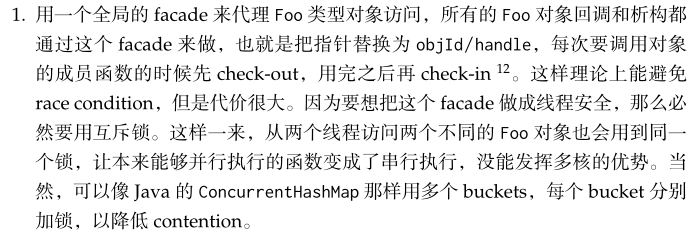
\includegraphics[width=360pt]{texlive2010.png}}}

\vspace{1ex}
\centerline{\fbox{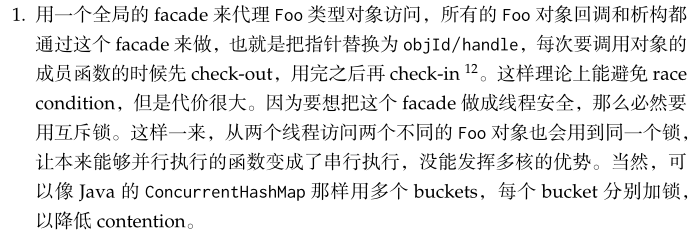
\includegraphics[width=360pt]{texlive2012.png}}}

\vspace{1ex}
因此我建议不要在排版期间升级 \LaTeX 的大版本,
这也是我在虚拟机上安装 TeX Live 的原因之一。
这样可以轻松地备份整个系统,
将来重印需要修订书中某几页的时候可以使用当年的虚拟机映像,版本一致,不必担心其他页面发生“动版”。

\subsection{PDF阅读器}
推荐SumatraPDF,它不锁PDF文件,可以随时覆盖,并且自动刷新。

\subsection{离线备份}
写书是一项耗时的任务,数据备份是必不可少的,
防止误操作和硬件损坏带来的不可弥补的损失。
除了 \S \ref{sec:versionControl} 讲的源文件版本管理之外,
各种图片、表格,以及生成PDF也要及时备份,
最好是离线(offline)备份。
可用以下这些网盘:

\begindot
\item Amazon Cloud Drive
\item Dropbox
\item Google Drive
\item Microsoft Sky Drive
\myenddot

这几个网盘都有Windows和Mac客户端,
这也是我使用Windows桌面的原因之一。

\section{版本管理}
\label{sec:versionControl}


我用Git管理 \fn{.tex} 文件和其他输入文件,
并且同步到 Github 的私人仓库,
就像这篇文章一样。

\subsection{理想的工作流程}
作者和编辑都使用版本管理软件,就像开发软件那样工作。
\LaTeX 就好比是编译器,
\fn{.tex} 文件是源程序,
\fn{.pdf} 文件是编译的结果。
作者和编辑都可以修改源程序,并且通过版本管理软件来merge结果。
考虑到作者和编辑不在同一个内网,因此一般要用公共的版本库,例如Github。
GitHub 的私有 repository 可保证数据安全。

\subsection{现实的工作流程}
编辑往往既不会\LaTeX也不会Git,那就之好采用原始方案,
作者提供PDF,编辑加以评注,或者打印出来再用红笔校对。

\section{\fn{.tex} 文件组织}
\fn{.tex} 文件一律使用 UTF-8编码,一来避免各种编码转换的问题(某些人名用字在GB2312中没有定义),
二来可以直接使用现有的Linux命令行工具来处理 \fn{.tex} 文件。
\fn{.tex} 文件一般可以按章或按节划分,每个文件不超过1000行,以利于编辑。
再用一个 \fn{.tex} 文件把它们 \mn{include} 到一起。
\fn{.tex} 和图片文件的文件名不要有下划线。

\chapter{样式}

\section{转义字符}
注意“\#\,”是 \TeX 元字符,因此 C\# 要写作 \fn{C\bs\#}。
类似的“\textasciitilde”也是元字符,
要写作\mn{textasciitilde}。
\index{命令!textasciitilde@\mn{textasciitilde}}
这两个字符在URL中也经常出现,要特别小心。

C/C++代码的标识符中经常出现下划线“_”,例如 \fn{boost::shared_ptr}、
\fn{random_\linebreak[0]shuffle} 等。
为了避免每次都转义,可以使用 \fn{underscore} 宏包,
将下划线变为普通字符。
\index{宏包!underscore@\fn{underscore}}
注意这里 \fn{random_\linebreak[0]shuffle} 在行尾断字,
那么下划线之后不应该出现连字号“-”,
因此应写为 \verb|random_\linebreak[0]shuffle|。

\section{斜体}
按照排版规范,数学变量名和(非标准)函数名应该用斜体,
常量、单位、标准函数名应该用正体。
例如:%$\footnote{c是真空中的光速,k是Boltzmann常数。}:
$n$-body 问题、%$E = m \mathrm{c}^2 、
%$V_\mathrm{T} = \frac{\mathrm{k} T}{q}$、
$\sin x = (\mathrm{e}^{\mathrm{i}x} - \mathrm{e}^{-\mathrm{i}x})/2\mathrm{i}$、
5\textmu s。
快速排序 $n$ 个元素的数度的平均时间复杂度是 $O(n \log n)$。
通过 TCP 发送 $n$ 字节的消息,
接收方收到这 $n$ 个字节的事件可能性有 $2^{n-1}$ 种
\footnote{在 $n-1$ 个字节间隙中,依次插入 $0, 1, \ldots, n-1$ 个“隔板”,
一共有 $C_{n-1}^0 + C_{n-1}^1 + \cdots + C_{n-1}^{n-1} = 2 ^ {n-1} $ 种情况。}。

\section{列表}
\LaTeX 默认的列表环境(\fn{itemize} 和 \fn{enumerate})是为多行文字准备的,
因此上下间距较大。我一般使用 \fn{enumitem} 宏包来重新定义列表环境,
并且定义几个简单的命令来使用它(\mn{begindot} 和 \mn{myenddot},\mn{beginnum} 和 \mn{myendnum})。
\index{宏包!enumitem@\fn{enumitem}}
\begin{Code}
\newcommand\begindot{\begin{itemize}
[itemsep=2pt plus 2pt minus 2pt,%
topsep=3pt plus 2pt minus 2pt,%
parsep=0pt plus 2pt minus 2pt]}
\newcommand\myenddot{\end{itemize}}
\end{Code}

\begin{Code}
\newcommand\beginnum{\begin{enumerate}
[itemsep=2pt plus 2pt minus 2pt,%
topsep=3pt plus 2pt minus 2pt,%
parsep=0pt plus 2pt minus 2pt]}
\newcommand\myendnum{\end{enumerate}}
\end{Code}

\section{章节标题}
章节标题无标点,因此 \S \ref{sec:whyTypesetting} 是错的。
\fn{ctex} 宏包默认会把章\mn{chapter} 和节\mn{section} 的标题居中,
这种样式显得很古板,章标题可以靠右,节标题和小节标题均靠左。
参见本文的\fn{format.cls} 文件。

\subsection{编号}
通常单个小节不编号,因此 \S \ref{subsec:noChineseItalic} 和本小节是错的。
应要改用\mn{subsection*} 命令。

\section{图表编号} %%%%%%%%%%%%%%%%%%%%%%%%%%%%%%

我不使用浮动环境,因此自己定义了 \mn{figcaption} 和 \mn{tabcaption} 命令来为图表编号。
图的标题位于下方,按章编号(图1-1、图1-2、图2-1 等等)。
例如

\begin{center}
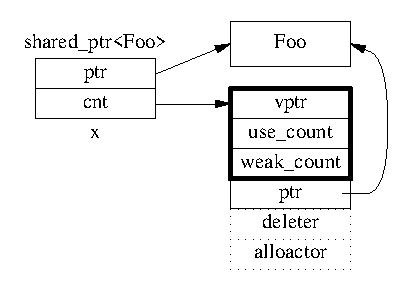
\includegraphics{sp0.eps}\\
\figcaption{\fn{shared_ptr} 的数据结构}\label{fig:sharedptr}
\end{center}


表的标题位于上方,按章编号(表1-1、表1-2、表2-1 等等)。
例如

\begin{center}
\tabcaption{水平空格命令的长度}

\vspace{1ex}
\begin{tabular}{ccl}
\hline
\textbf{命令} & \textbf{长度} & \textbf{用途}\\
\hline
\mn{quad} & 10pt & 图表编号与图表标题之间的全角空格\\
\mn{,} & 1.67pt & 千分空,例如 65\,536\\
\hline
\end{tabular}
\end{center}

\section{脚注} %%%%%%%%%%%%%%%%%%%%%%%%%%%%%%

\subsection{编号}
\LaTeX 默认是按章重置脚注编号,
这么如果重印的时候需要增加一个脚注,
势必会影响后续页码,这是 \mybooktitle 排版的一个教训。
因此我意识到脚注应该是按页重置,但是 \verb|\@addtoreset{footnote}{page}|
无效,必须使用 \fn{footmisc} 宏包的 \fn{perpage} 选项,
例如 \sfn{\bs usepackage[perpage]\{footmisc\}}。
\index{宏包!footmisc@\fn{footmisc}}

\LaTeX 默认的脚注编号是数字,这有时会造成误解。
例如给长度单位pt添加脚注,正文中可能会出现“pt\textsuperscript{2}”,
让人误以为是面积单位,因此可以改用带圈数字。

\subsection{置底}
\LaTeX 默认的脚注位置不是固定置底,而有可能随页面内容而浮动。例如 \myurl{footnote-middle.tex}。

\vspace{1ex}
\centerline{\fbox{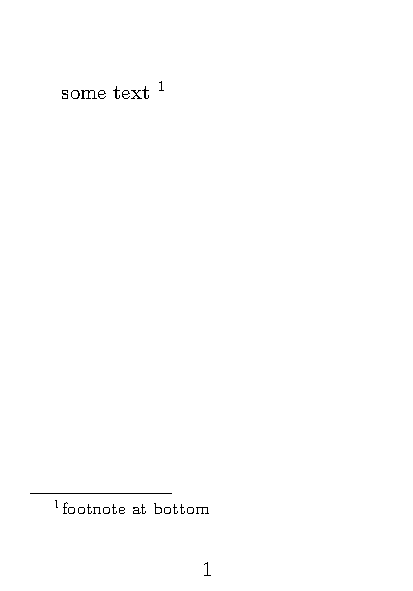
\includegraphics[page=1]{footnote-middle.pdf}}%
\quad\fbox{\includegraphics[page=2]{footnote-middle.pdf}}}

使用 \fn{footmisc} 宏包的 \fn{bottom} 选项之后,
脚注置底。见 \myurl{footnote-bottom.tex}。 \nopagebreak

\vspace{1ex}
\centerline{\fbox{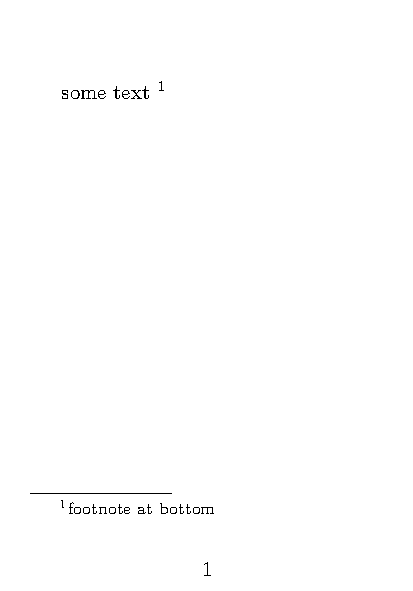
\includegraphics[page=1]{footnote-bottom.pdf}}%
\quad\fbox{\includegraphics[page=2]{footnote-bottom.pdf}}}

\section{参考文献}
技术书籍不是学术著作,可不必使用 BibTeX 工具,直接按出版社的格式要求排版参考文献即可。

\chapter{规则}


\section{章节编号}

\section{阿拉伯数字}

飞流直下3000尺,疑似银河落9天。

\section{全角与半角}

\section{参考文献}


\chapter{微调}
\myurl{http://www.economics.utoronto.ca/osborne/latex/PMAKEUP.HTM}

\section{分段与分页}

\section{阿拉伯数字}

飞流直下3000尺,疑似银河落9天。

\section{全角与半角}

\section{参考文献}


\chapter{工具}
《Linux多线程服务端编程——使用muduo C++网络库》这本书是我自己用 \LaTeX 排版的,
在排版过程中也积累了一些小工具,本章把它们一一展示出来。
不少工具都直接基于开源的 iText PDF 库,可从 \myurl{http://itextpdf.com/} 下载,
我用的是 \fn{itextpdf-5.3.0.jar}。另外一些则用到了 Ghostscript,
可直接用 \fn{apt-get} 安装。

\subsubsection{下载}

Groovy 版本位于 \myurl{https://github.com/chenshuo/typeset/tree/master/tools}

Java 版本位于 \myurl{https://github.com/chenshuo/recipes/tree/master/java/pdf}

各个工具的输出示例位于 \myurl{http://vdisk.weibo.com/s/kT4fL}

\section{统计中文字数}
\LaTeX 没有像 Word 那样自带中文字数统计功能,加上 \LaTeX 源文件中有许多控制字符,
不能通过文件大小准确获知其中有多少汉字。
为此我用C写了一个统计中文字数的小工具,名为 \fn{cwc},即 chinese word counter,
这个工具可以处理GBK、Unicode (UCS-2)、UTF-8这三种编码的文件。\mpar{补例子}
源码位于 \myurl{https://github.com/chenshuo/recipes/tree/master/utility}。
以下是一次运行的输出。
\index{工具!cwc@\fn{cwc}}
\begin{Code}
$ cwc chapTools.tex chapRules.tex
   119   1012    5329 chapTools.tex (UTF-8)
    13     33     167 chapRules.tex (UTF-8)
   132   1045    5496 total
  行数   字数   字节数
\end{Code}

\section{PDF内容对比(dif\/f\,)}
在书籍出版之后,每次印刷都可能修订一些内容,
在把新的PDF文件交给出版社的同时,也要通知哪些页码有改动,
方便出版社印刷。
由于PDF是二进制格式,无法直接对比新旧PDF文件,
于是我写了一个 \fn{diffpdf.sh} 小工具用来找出哪些页面的内容有改动。
这个工具的思路很土,就是先用 Ghostscript 把PDF按页渲染为多个PNG文件,
然后用 \fn{diff(1)} 比较新旧两个PDF渲染出来的这些PNG文件是否相同。
然后用 Python 脚本(\fn{diffpng.py})将两个PNG文件的不同之处用红色高亮显示出来。例如:
\index{工具!diffpdf@\fn{diffpdf.sh}}
\index{工具!diffpng@\fn{diffpng.py}}

\vspace{1ex}
\centerline{
\includegraphics{diffpng.png}}

\section{PDF截取}
为了在网上公布样张,我需要从整书中截取一部分页码,
另存为PDF文件,这用 \fn{pdftk} 最方便了。
例如
\index{工具!pdftk@\fn{pdftk}}

\begin{Code}
pdftk book.pdf cat 1-16 output preamble.pdf     # 前言和目录
pdftk book.pdf cat 19-46 output chap1.pdf       # 第1章
pdftk book.pdf cat 577-end output appendix.pdf  # 附录
\end{Code}


\section{PDF页码编号}

\LaTeX 的 \fn{hyperref} 宏包可以为生成的PDF设置“逻辑页码”,
例如前言目录用罗马数字,正文用阿拉伯数字。
不过经过 \fn{pdftk} 截取之后就失效了。
为此我编写了 \fn{pagenum.groovy} 工具,用来添加逻辑页码。例如
\index{工具!pagenum@\fn{pagenum.groovy}}

\begin{Code}
pagenum.groovy '1e,3r' preamble.pdf  # 第1、2页是封面,没有页码;第3页开始用罗马数字
pagenum.groovy '1n3'   chap1.pdf     # 第1章第1页的逻辑页码是3
pagenum.groovy '1n561' appendix.pdf  # 附录第1页的逻辑页码是561
\end{Code}


\section{PDF剪裁(crop)}
为了充分利用屏幕空间,也便于在电子阅读器(iPad、Kindle)上阅读校对书稿,
我一般会把PDF剪裁为版心大小。
例如下面左图是原始PDF,为纸张大小;右图是按固定Crop Box剪裁之后的版心。
\mpar{固定剪裁}
\index{工具!crop@\fn{crop.groovy}}

\vspace{1ex}
\centerline{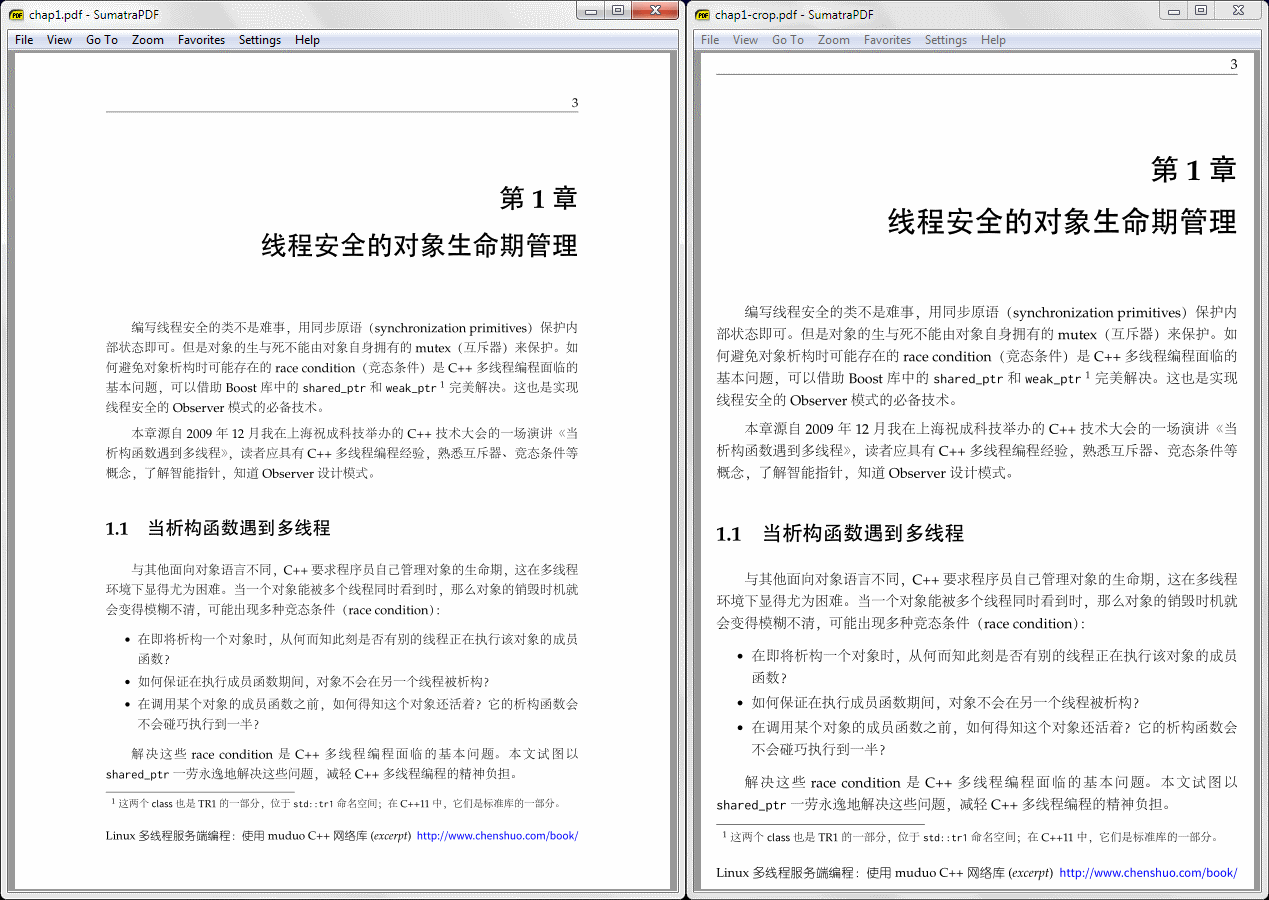
\includegraphics[scale=0.4]{crop.png}}

剪裁工具是 \fn{crop.groovy},设好 \sfn{CLASSPATH} 后可直接在命令行运行。
其核心是根据版心和纸张尺寸算出左下角和右上角左边,然后剪裁每一页。
这个工具不管PDF的内容,如果需要根据页面内容剪裁PDF,\mpar{按内容剪裁}
可以使用Heiko Oberdiek编写的 \fn{pdfcrop} 工具,地址如下:
\index{工具!pdfcrop@\fn{pdfcrop}}

\begindot
\item \myurl{http://www.ctan.org/tex-archive/support/pdfcrop}
\item \myurl{http://code.google.com/p/pdfcrop2/}
\myenddot

%\subsection


\section{PDF拼接(two-up)}
有时候想在宽屏上同时阅读左右两页的书稿,除了可以用PDF阅读器本身的多页显示功能,
我还常常自己做二合一(two-up)。
这样得到的PDF也可以打印出来看,既节约纸张,而且与原稿是1:1大小。生成的PDF效果如下图。
\index{工具!twoup@\fn{twoup.groovy}}

\vspace{1ex}
\centerline{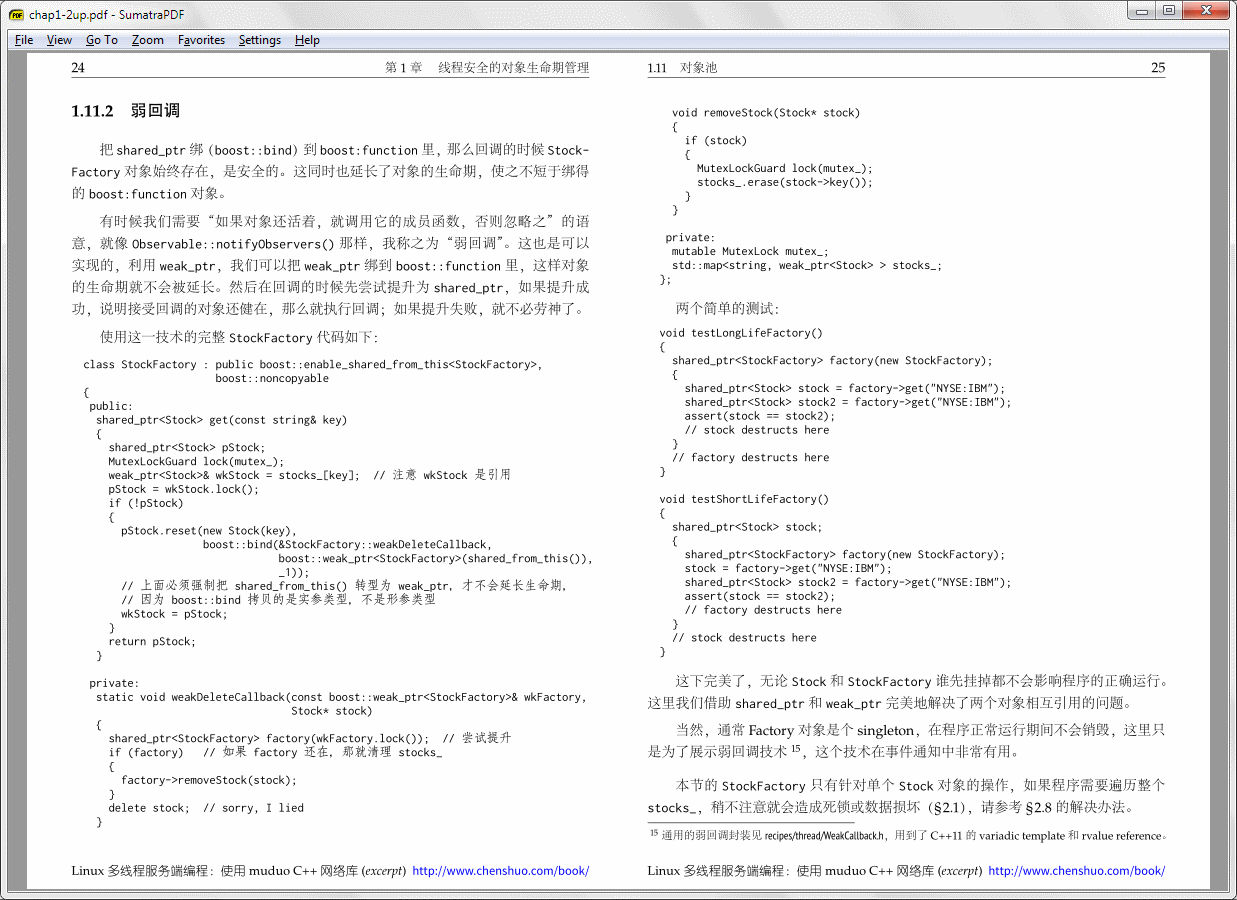
\includegraphics[scale=0.4]{twoup.png}}

二合一工具是 \fn{twoup.groovy},其核心是算出左右两页在合页中的起始坐标。

\section{PDF小册子(booklet)}
\index{工具!booklet@\fn{booklet.groovy}}
有时候我会把一章的内容打印出来,装订成一本小册子,这样读起来有翻书的感觉。
为了节约纸张,在打印之前要拼版,这样一张纸双面能打印4个页码。
例如8页内容可以打印到两张A4纸上:

\vspace{1ex}
\centerline{\includegraphics{booklet-1.eps}\qquad\includegraphics{booklet-2.eps}}

对折、叠好,骑缝订之后就是一本小册子了。

\begin{center}
第一张纸的正反两面打印:\nopagebreak

\vspace{1ex}
\includegraphics{booklet-3.eps}\qquad\includegraphics{booklet-4.eps}

\vspace{1em}
第二张纸的正反两面打印:

\vspace{1ex}
\includegraphics{booklet-5.eps}\qquad\includegraphics{booklet-6.eps}
\end{center}

小册子工具是 \fn{booklet.groovy},其核心是算出每面纸应该放哪两个页码的原始内容。

装订这种小册子要用骑缝订,可用旋转订书机
\footnote{\myurl{http://www.amazon.cn/dp/B0080AF0FM} \quad \myurl{http://product.dangdang.com/product.aspx?product_id=1141537002}}。
一本小册子一般应该控制在10页纸左右,即40个页码,再厚就订不透了。

\section{PDF字体嵌入}
出版社拿到作者提供的终稿PDF之后,如果没有进一步修改,就会准备印刷了。
第一步是让出片公司打印出胶片,即“出片”。
这种公司使用的操作系统很可能与作者不同,特别是安装的字体可能不一致。
为了防止出现文字乱码或字体错乱,出片公司一般都会要求提供嵌入全部字体的PDF文件。

\begin{Codex}[label=/usr/share/ghostscript/???/Resource/Init/gs_pdfwr.ps]
/.standardfonts [
%  /Courier /Courier-Bold /Courier-Oblique /Courier-BoldOblique
%  /Helvetica /Helvetica-Bold /Helvetica-Oblique /Helvetica-BoldOblique
%  /Times-Roman /Times-Bold /Times-Italic /Times-BoldItalic
%  /Symbol /ZapfDingbats
] readonly def
\end{Codex}


\appendix % 开始附录,章用字母编号


\end{document}
